\documentclass[exam,addpoints,noanswers]{exam}

\usepackage[exam]{biology11}

\title{Test \#4 (earned honors)}
\date{\printdate{6/1/2021}}
\author{\mobeardInstructorShort}

\begin{document}
\maketitle
\vfill
\mobeardExamNameBlock
\vfill
Instructions: 
\begin{enumerate}
\item Do not open exam until instructor announces that you may begin.
\item Closed notes, closed book.  You may use two \SI{8.5x11}{\inch} hardcopy note sheets, both sides. You may \textbf{not} use your computer or phone as your notes. 
\item Please write your name on each page in case the sheets are separated. 
\item Multiple choice/short answer are worth one point, essay questions are worth substantially more. I recommend you quickly read through the multiple choice/short answer questions and use the information contained within them to aid you in answering the essay questions, but do not spend excessive time answering the multiple choice. If time permits, please answer all before turning in your test to maximize your score.
\item In answering the short answer questions, be thorough but concise. Deep understanding of the concepts will be displayed by proper use of vocabulary and discussion of the interconnectedness of concepts.
\end{enumerate}
\vfill
\begin{center}
\gradetable[h][questions]
\end{center}
\clearpage

\begin{questions}
\question[1] What is mitosis? 
\begin{solution}[\fill]
A process by which a diploid nucleus splits into two identical diploid nuclei. 
\end{solution}

\question[1] What are the phases of mitosis in the correct order?
\begin{solution}[\fill]
prophase, metaphase, anaphase, telophase
\end{solution}

\question[1] Wich of the following are correct? Select all that apply.
\begin{choices}
\CorrectChoice During prophase I, the chromosomes condense. 
\CorrectChoice During metaphase II, the chromosomes line up along the equator.
\CorrectChoice During anaphase I, the nuclear membrane dissolves.
\CorrectChoice During anaphase II, the chromosomes are split and pulled along the spindle towards opposite poles.
\CorrectChoice During telophase II, the nuclear membrane re-forms, resulting in four daughter nuclei.
\end{choices}

\question[1] What is meiosis? 
\begin{solution}[\fill]
A process by which a diploid nucleus splits into four non-identical haploid nuclei.
\end{solution}

\clearpage
\begin{figure}[th]
\begin{center}
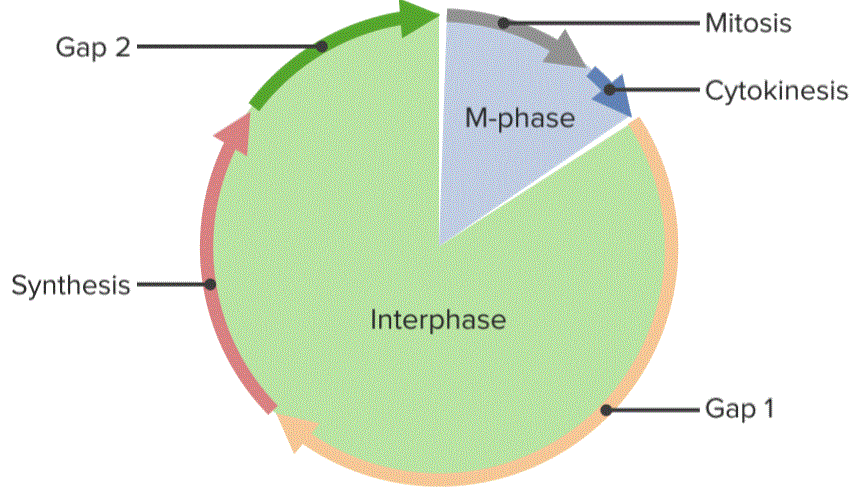
\includegraphics[width=3in]{cellcycle.png}
\end{center}
\caption{Cell cycle, divided into five phases. From \url{https://www.lecturio.com/magazine/the-cell-cycle/}}
\label{fig:cellcycle}
\end{figure}

\question[1] Please refer to \fref{fig:cellcycle}. Which of the following takes place during the portion labeled Gap 1 (G1) phase? Please select all that apply. 
\begin{choices}
\CorrectChoice Growth.
\CorrectChoice Respiration.
\CorrectChoice Doing ``normal'' things that a cell might be specialized/differentiated for.
\CorrectChoice Moving things across the cell membrane. 
\choice Replication of DNA. 
\end{choices}

\question[1] Please refer to \fref{fig:cellcycle}. During which phase does DNA replication occur? 
\begin{choices}
\choice Gap 1
\CorrectChoice Synthesis
\choice Gap 2
\choice Mitosis
\choice Cytokinesis
\end{choices}

\question[1] Please refer to \fref{fig:cellcycle}. Which of the following takes place during the portion labeled Gap 2 (G2) phase? Please select all that apply. 
\begin{choices}
\CorrectChoice Synthesis of proteins etc that are needed to enable or guide cell division.
\choice Regular ``vanilla'' growth.
\choice Replication of DNA.
\choice Phagocytosis.
\choice Apoptosis.  
\end{choices}

\clearpage
\question[1] Which of the following statements regarding evolution is \textbf{FALSE}?
\begin{choices}
\CorrectChoice Evolution has a ``drive'' and always acts to improve performance.
\choice Evolution is descent with modification.
\choice Evolution is a consequence of having heritable traits and differential survival of offspring.
\choice Evolution occurs over geologic timescales, but can also occur rapidly such as in COVID-19.
\end{choices}

\question[1] Based on \emph{scientific evidence}, approximately how old is life on earth?
\begin{choices}
\CorrectChoice Prokaryotic life is around 3.9 billion years old, multicellular organisms have only been around for about 500 million years.
\choice 5000 years.
\choice 17 years.
\choice Everything is 1 day old and was created yesterday by an evil genius out to trick us. 
\end{choices}

\question[1] The alternative forms of a gene are known as
\begin{choices}
\choice isomers. 
\choice crossovers. 
\choice translocations. 
\CorrectChoice alleles. 
\choice none of these.
\end{choices}





% Essay section
\clearpage
\question
\begin{parts}
\part[20]\label{part:11a} Please explain, using both text and drawings, two ways that meiosis generates genetic variation.  
\begin{solution}[\fill]
(1) Independent assortment, shuffling what alleles are present; and (2) recombination during crossover. 
\end{solution}
\part[2] Contrast your answer in part~\ref{part:11a} with asexual reproduction (e.g. by mitosis only): how is genetic variation generated in asexual reproduction? 
\begin{solution}[\fill]
In asexual reproduction, mutation is the main (only?) way to generate genetic variation.
\end{solution}
\end{parts}

\clearpage
\question[23] If mice with normal ears (wild type) are crossed with mice with twisted ears, all the $f_1$ progeny have normal ears. Using a Punnett square, predict the phenotype of the $f_2$ progeny and their relative proportions.
\begin{solution}
Since no mice with twisted ears appear as a result of the $P_1$ cross, we will assume the parents were homozygous. Since all $f_1$ progeny had normal ears, we will also assume that normal ears ($T$) are dominant over twisted ears ($t$). The $f_1$ progeny, being heterozygous ($Tt$), will produce both $T$ and $t$ gametes in equal numbers. Therefore, the Punnett square for the f1 cross would be:
\begin{center}
\begin{tabular}{|c|c|c|}
\hline
& T & t \\
\hline
T & TT &Tt \\
\hline
t & Tt & tt \\
\hline
\end{tabular}
\end{center}
Since $T$ is dominant over $t$, all genotypes containing even one $T$ will have normal ears; only $tt$ genotypes will express the wrinkled-wing phenotype. Thus, the $f_2$ progeny will show a typical Mendelian dominant-recessive relationship of 3:1.
\end{solution}

\clearpage
\question[23] Sketch what you expect to see when observing meiosis. Make several sketches, one for each of the phases we discussed. Please number them or make clear what order they are in. For each, label important structures and add a caption explaining the action happening. 

\clearpage
\question A black labrador (Maura), from a long line of only black labradors, is bred with a chocolate (brown) labrador (Rollo) from a long line of only chocolate labradors. 
\begin{parts}
\part[5] What are the most likely genotypes and phenotypes of Maura and Rollo? Please explain your reasoning. 
\begin{solution}[\fill]
Maura is $BB$; Rollo is $bb$. There is also an $E$ gene but since they both come from lines that ``breed true'' we may assume both parents are homozygous dominant $EE$. 
\end{solution}
\part[5] Draw a Punnet square for the $f_1$ generation. 
\begin{solution}[\fill]
\begin{center}
\begin{tabular}{|c|c|c|}
\hline
& b & b \\
\hline
B & Bb & Bb \\
\hline
B & Bb & Bb \\
\hline
\end{tabular}
\end{center}
\end{solution}
\part[5] Draw a Punnet square for the $f_2$ generation. 
\begin{solution}[\fill]
\begin{center}
\begin{tabular}{|c|c|c|}
\hline
& B & b \\
\hline
B & BB & Bb \\
\hline
b & Bb & bb \\
\hline
\end{tabular}
\end{center}
\end{solution}
\part[5] Please give the expected proportions for the genotypes and phenotypes in the $f_2$ generation. 
\begin{solution}[\fill]
In the $f_2$ generation, we expect to see 1 $BB$: 2 $Bb$ : 1 $bb$, or 3 black : 1 chocolate. 
\end{solution}
\part[2] Would your results hold in general, for any black labrador and chocolate labrador mating? 
\begin{solution}[2em]
No, if the dogs were any black or chocolate lab, they may not be homozygous dominant for the $E$ gene and thus we might see yellow labs in $f_1$ and $f_2$.  The action of the $E$ gene is an example of epistasis. 
\end{solution}
\end{parts}


\end{questions}
\end{document}